\documentclass{article}

\usepackage{graphicx}
\usepackage{listings}
\usepackage{hyperref}

\hypersetup{
    colorlinks=true,
    linkcolor=black,
    filecolor=magenta,      
    urlcolor=blue,
    pdftitle={Tecnologie internet},
    pdfpagemode=FullScreen,
    }



\begin{document}
    \author{dmotrio}
    \title{Tecnologie internet}
    \date{2021}

    \maketitle
    \tableofcontents
    \listoffigures
    \listoftables

    \section{Tecnlogie internet}
    \subsection{HTTP}
\subsubsection{Network protocols}
Un protocollo è la definizione del comportamento fra due entità che devono comunicare.
\subsubsection{Protocols layer}
Le fuzioni del network sono strutturate con un modello layer, i dati scambiati fra i layer prendo il nome di SDU(Service Data Protocol).
I dati che vengono scambiati fra uno strato protocollare ad un'altro prendo il nome di PDU(Protocol Data Unit).

\subsubsection{TCP(Transmission Control Protocol)}
\begin{itemize}
    \item Trasporto affidabile
    \item controllo del flusso
    \item controllo della congestione
    \item connection-oriented
    \item non fornisce: timing, sicurezza e minimumvthroughput guarantee
\end{itemize}

\subsubsection{UDP(User Datagram Protocol)}
\begin{itemize}
    \item Trasferimento non affidabile
\end{itemize}

\subsubsection{HTTP overview}
Http usa un modello client server, con le seguenti caratteristiche:
\begin{itemize}
    \item user agent: client manda richieste al server(browser, bot, ecc)
    \item origin server: programma che accetta o rifiuta le richieste
    \item local cache: memoria locale(possonoaverla sia il client che il server)
    \item proxy: applicazione intermediaria che svolge il compito sia di client che di server
    \item gateway: applicazione intermediaria(non conosciuta dal client) che permette di nascondere le specifiche del server
\end{itemize}

HTTP usa TCP e sfruttano la porta 80, HTTP non mantiene informazioni riguardo richieste passate del client.
Le connessioni che permette HTTP possono essere persitenti o non, nel caso delle connessioni non persitenti, dopo ogni invio di dati, la connessione viene chiusa.
Nel caso delle connessioni persistenti(Invio di un file grande come un video) la connessione rimane aperta fino all'accertato invio delle risorse.

Per velocizzare l'invio e la ricezione dei pacchetti, si ricorre al pipelining, al posto di inviare un pacchetto ed aspettare la notifica di avvenuta ricezione, con il pipelining si invia i pacchetti in blocchi per ridurre il tempo complessivo.

\subsubsection{Messaggio HTTP}
Il messaggio HTTP è composto di un header e un body, l'header viene popolato da:
\begin{itemize}
    \item caratteristiche di transmissione generali
    \item caratteristiche dell'entità di transmissione
    \item caratteristiche richieste
    \item caratteristiche di risposta
\end{itemize}

Esempio di richiesta HTTP:

\begin{lstlisting}
    GET /index.html HTTP/1.1\r\n
    Host: www-net.cs.umass.edu\r\n
    User-Agent: Firefox/3.6.10\r\n
    Accept: text/html,application/xhtml+xml\r\n
    Accept-Language: en-us,en;q=0.5\r\n
    Accept-Encoding: gzip,deflate\r\n
    Accept-Charset: ISO-8859-1,utf-8;q=0.7\r\n
    Keep-Alive: 115\r\n
    Connection: keep-alive\r\n
    \r\n
\end{lstlisting}

N.B. \textbackslash r\textbackslash n è la combinazione per andare a capo e, se usata senza altro testo, ha lo scopo di seprare le varie parti del pacchetto come request, header e body.


\subsubsection{Metodi HTTP}
\begin{itemize}
    \item GET: trasferisce la risorsa
    \item HEAD: trasferisce solo l'header
    \item POST: effettua un processo risosa-specifico sul payload
    \item PUT: rimpiazza tutte le rappresentazioni di una certa risorsa
    \item DELETE: elimina tutte le rappresentazioni di una certa risorsa
    \item CONNECT: stabilisci la connessioni con il server
    \item OPRIONS: descrivi le opzioni della comunicazione
    \item TRACE: fai un messsage loop-back
\end{itemize}

\subsubsection{Messaggi HTTP idempotenti e sicuri/non sicuri}
\begin{itemize}
    \item idempotente: Metodo che se chiamato una o cento volte fornisce sempre lo stesso risultato
    \item sicuro: metodo che non modifica la risorsa(GET e POST ecc)
\end{itemize}

\subsubsection{Metodi}
\begin{itemize}
    \item GET: \textbf{Sicuro e idempotente}, usato per richiedere una risorsa
    \item POST: \textbf{Non sicuro e nemmeno idempotente}(perche ripetere la stessa azione porta a creare duplicati), usato per creare/aggiornare una risorsa
    \item PUT: \textbf{Idempotente ma non sicuro}, usato per aggiornare o creare una risorsa
    \item DELETE: \textbf{Idempotente ma non sicuro}, elimina le risorse specificate
    \item HEAD: \textbf{Sicuro e idempotente}, usato per richiedere l'header di una risorsa.
    Usato per controllarer la validità di un URL, ecc
\end{itemize}

\subsubsection{Caratteristiche dell'header HTTP}
\begin{itemize}
    \item User-agent: Descrive il client che ha fatto la richiesta
    \item Referer: URL del'elemento dal quale arriva la richiesta URL
    \item Host: Dominio e porta ai quali fare la richiesta
    \item From: utilizza la mail e l'user-agent della persona che fa la richiesta
    \item Range: specifica la grandezza della risorsa(utile nei download)
    \item Accept, Accept-Charset, Accept-Encoding, Accept-Language: formati di negoziazione per permettere al client e al server di usare le stesse Tecnologie.
    \item If-Modified-Since, If,Unmodified-Since: usato nelle richieste HTTP condozionali!!
    \item Authorization, Proxy-Authorization
\end{itemize}

\subsubsection{Codici di stato per HTTP}
\begin{itemize}
    \item 1xx - informazionale
    \item 2xx - successo
    \item 3xx - reindirizzato
    \item 4xx - errore del client
    \item 5xx - errore del server
\end{itemize}

\subsubsection{Cookies}
I Cookies vengono solitamente utilizzati per autenticazione, carrelli della spesa, raccomandazioni e mantenimento dello stato dell pagina web.


\begin{figure}[h!]
	\centering
	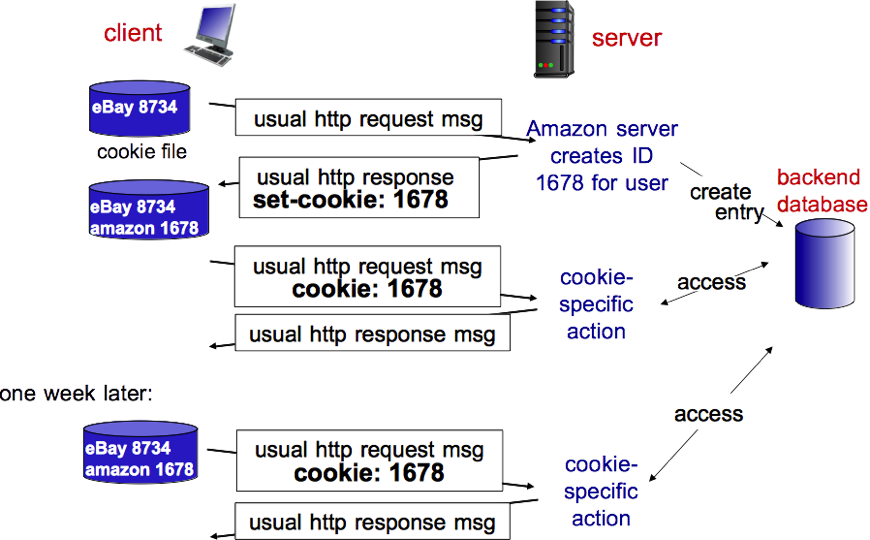
\includegraphics[width=0.6\linewidth]{imgs/1 - cookies.png}
	\caption{Cookies}
	\label{fig:Cookies}
\end{figure}

\subsubsection{Proxy}
Un proxy è un intermediario che ha sia funzioni client che server.
\subsubsection{Web caching}
\begin{figure}[h!]
    \centering
    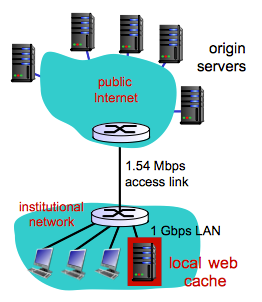
\includegraphics[width=0.3\linewidth]{imgs/2 - web cache.png}
    \caption{Esempio di web caching}
    \label{fig:WebCache}
\end{figure}
    \subsection{Apache server HTTP}
\begin{figure}[h!]
    \centering
    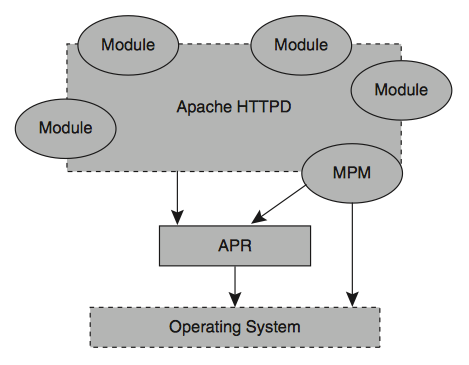
\includegraphics[width=0.5\linewidth]{imgs/3 - apache modules.png}
    \label{fig:apache}
    \caption{Architettura apache HTTPD}
\end{figure}
Apache HTTPD server si appogia al sistema operativo mediante l'APR(Apache Portable Runtime) e mediante moduli permette il fornimento di servizi web.

    \subsection{HTML}
Linguaggio di markup per rappresentare documenti nel web.

    \subsection{CSS}
Il css vine utilizzato per applicare stile ai documenti HTML.

    \subsection{XML}
EXtensible Markup Language viene utilizzato per trasportare informazioni, viene utilizzato nei documenti HTML per arricchire il contenuto mediante dati dinamici.

    \subsection{JSON}
Moderna versione di XML, rappresenta gli oggetti nel linguaggio di scripting JavaScript.

Un documento json rappresenta i dati in una maniera più leggibile di xml.
\begin{lstlisting}
{"employees":[
    {
        "firstName":"John",
        "lastName":"Doe"
    },
    {
        "firstName":"Anna",
        "lastName":"Smith"
    },
    {
        "firstName":"Peter",
        "lastName":"Jones"
    }
]}
\end{lstlisting}
Al posto di:
\begin{lstlisting}
<employees>
    <employee>
        <firstName>John</firstName> <lastName>Doe</lastName>
    </employee>
    <employee>
        <firstName>Anna</firstName> <lastName>Smith</lastName>
    </employee>
    <employee>
        <firstName>Peter</firstName> <lastName>Jones</lastName>
    </employee>
</employees>
\end{lstlisting}
    \subsection{Search Engine for the Web}
\subsubsection{Web search}
L'operazione di ricerca nel web è molto simile al ricevere informazioni specifiche da un determinato server, solo che utilizza il linguggio naturale per cercare i documenti html.
\subsubsection{Motori di ricerca}
I motori di ricerca hanno tre caratteristiche principali:
\begin{enumerate}
    \item Crawling:
        navigare in internet per cercare tutti i contenuti
    \item Indexing
        salvare e organizzare tutti i documenti trovati durante il Crawling
    \item Ranking
        riorganizzare i risultati della ricerca in base all'accuratezza nel rispondere al'argomento ricercato(se cerca cane, non mi aspetto di trovare navi militari ecc)
\end{enumerate}

L'indice di tutti i documenti deve essere regolarmente aggiornato per includere nuove pagine.

\subsubsection{Web crawling}
Un crowler basilare(robot, bot, spider) consiste in:
\begin{itemize}
    \item Una coda di URI da visutare
    \item Un metodo per ricevere le risorse delle pagine con HTTP
    \item Un page parser per estrarre informazione
    \item Una connessione all'indicizzatore del motore di ricerca
\end{itemize}
Il procedimento ordinario consiste in: prendere un URL, analizzare e trovare URL all'interno del testo per aggiungere questi link nella coda di analisi e continuare a indicizzare le pagine.

\subsubsection{PageRank}
Algoritmo per il page ranking inventato da Larry Page, utilizzato da Google per il suo motore di ricerca.
PageRank è un algoritmo che analizza i link fra le risorse e il risultato viene utilizzato per il ranking.
Avendo una pagina $p$ e questa pagina è collegata alle pagine $q_1, ..., q_n$.
\begin{displaymath}
    PR(p) = (1-d) + d[\frac{PR(q_1)}{C(q_1)}+ ... + \frac{PR(q_n)}{C(q_n)} ]
\end{displaymath}
    \subsection{JavaScript - Basics}
\subsubsection{Incorporare JS in HTML}
\begin{lstlisting}[language=html]
<!DOCTYPE html>
<html>
    <body>
    <h1>My Web Page</h1>
    <p id="demo">A Paragraph</p>
    <button type="button" onclick="myFunction()">Try it</button>
    <script>
        function myFunction() {
        document.getElementById("demo").innerHTML = "Paragraph changed.";
        }
    </script>
    </body>
</html>
\end{lstlisting}
Solitamente si preferisce includere il documento JS a parte e poi importarlo con delle chiamate nel documento HTML.

\subsubsection{Parole riservate per JavaScript}
\begin{figure}[h!]
    \centering
    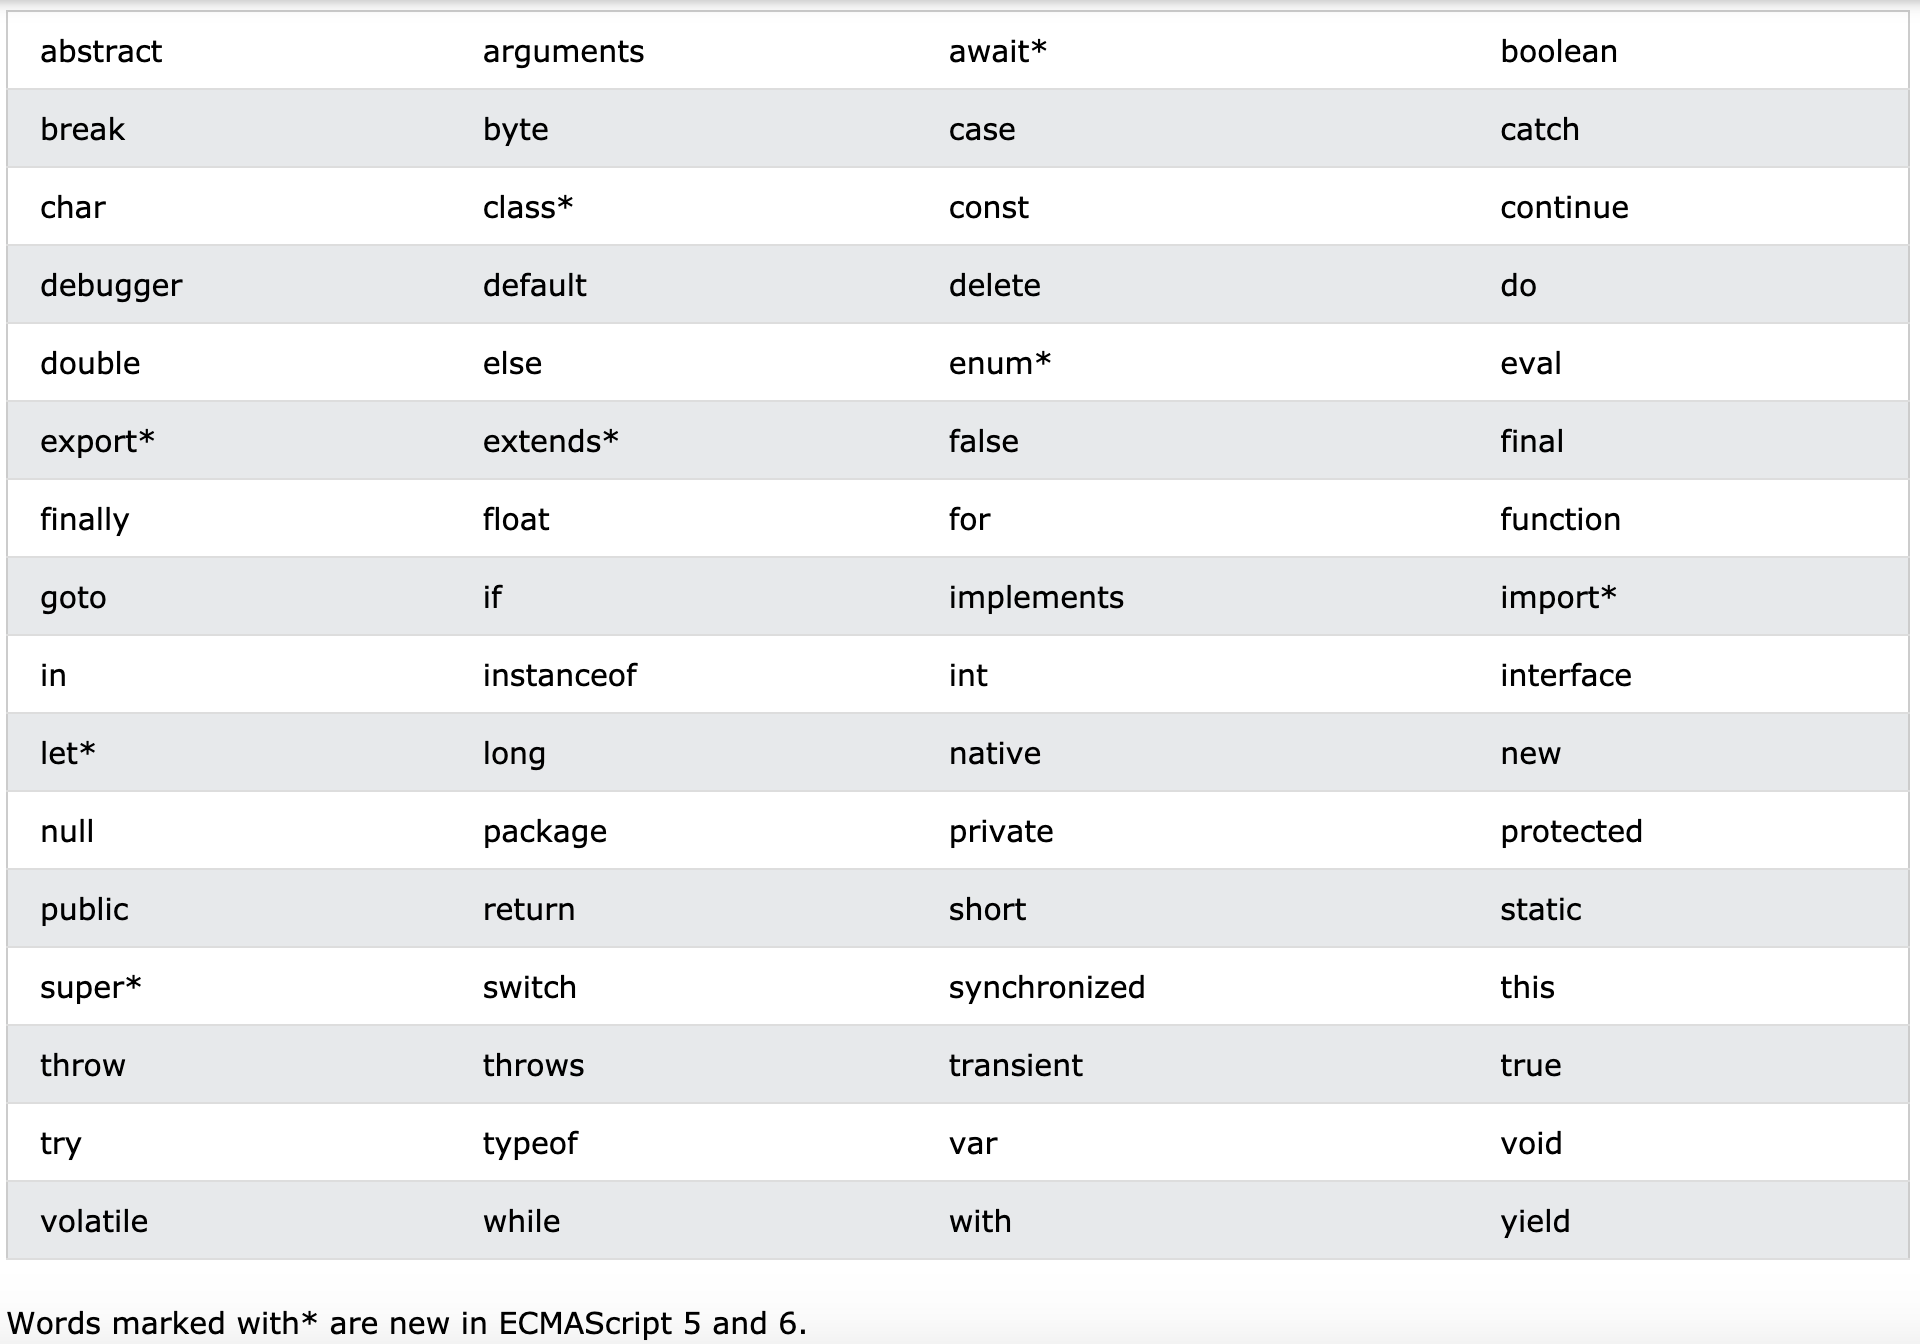
\includegraphics[width=0.8\linewidth]{imgs/4 - reserved keyword.png}
    \label{fig:ReserverKeyword}
    \caption{Parole riservate in JS}
\end{figure}

\subsubsection{Costanti e variabili}
Si usa \textbf{const} per le costanti e \textbf{let} per le variabili.

\subsubsection{Funzioni}
\begin{lstlisting}
function myFunction(p1, p2) {
    return p1 * p2;
}
\end{lstlisting}
\subsubsection{ArrowFunction}
\begin{lstlisting}
    const sum = (x, y) => { return x + y; };
\end{lstlisting}
\subsubsection{Oggetti}
\begin{lstlisting}
let person = {
    firstName:"John",
    lastName:"Doe",
    age:50,
    eyeColor:"blue",
    fullName:function() {return this.firstName + " " + this.lastName;}
};
\end{lstlisting}
Si può accedere ad un oggetto in due modi:
\begin{itemize}
    \item objectName.propertyName
    \item objectName[propertyName]
\end{itemize}
Per accedere ai metodi: objectName.methodName()


    \subsection{JavaScript Execution Window DOM}
\subsubsection{Client Side JS timeline}
\begin{enumerate}
    \item Il browser web crea un oggetto documento e comincia a fare il parsing del documento HTML, la proprietà \textit{document.readyState = loading}.
    \item Quando il parser incontra un tag script senza async o defer, scarica lo script e lo eseguisce come se fosse uno script in linea
    \item Quando il parser incontra script che hanno attributi come async o defer, semplicement scarica gli script ma non esegue nulla, continua con il parsing della pagina
    \item quando tutto il documento ha finito il parsing, \textit{document.readyState = interactive}
    \item Ogni script che ha l'attributo defer, vine eseguito nell'ordine con il quale appaiono nel documento
    \item Il browser accende l'evento \textit{DOMContentLoaded} nel document object, che rappresenta la transiziona dagli script sincroni a quelli asincroni
    \item quando tutta la pagina è stata caricata, compresi tutti gli script async, \textit{document.readyState = complete}
\end{enumerate}

\subsubsection{Same-origin policy}
Politica per la quale JavaScript, può interagire solo con il codice della sua finestra del browser, come se fosse in un sandbox(container ecc), per motivi di sicurezza.

\subsubsection{Window Object}
Le sue proprietà principali solo legate a:
\begin{enumerate}
    \item timers: permette di schedulare una funzione dopo un'intervallo di tempo.
    \item browser location e navigation: rappresenta l'URL corrente.
    \item browser history
    \item browser and screen info: Browser vendor e version number
    \item dialog boxes: Semplici box di dialogo
    \item document element: ogni elemento dell'HTML che ha un id può essere selezionato con questo oggetto.
    \item cross-window comunication
\end{enumerate}

\subsubsection{DOM}
DOM sta per Document Object Model e viene usato per prendere, modificare e aggiungere elementi HTML.

\subsubsection{Esempio DOM}
\begin{lstlisting}
<html>
<body>
<p id="demo"></p>
<script>
document.getElementById("demo").innerHTML = "Hello World!";
</script>
</body>
</html>  
\end{lstlisting}

    \subsection{Client-side JavaScript}
\subsubsection{Gestione eventi}
\begin{itemize}
    \item onchange
    \item onclick
    \item onmouseover
    \item onmouseset
    \item onkeydown
    \item onload
\end{itemize}
\subsubsection{AJAX - Asynchronous JavaScript and XML}
AJAX permette alla pagina di essere aggiornata in maniera asincrona senza aggiornare la pagina.

    \subsubsection{JQuery}
JQuery è una libreria che ha lo scopo di semplificare l'uso di JavaScript.
JQuery ha le seguenti funioni:
\begin{itemize}
    \item HTML/DOM manipulation
    \item CSS manipulation
    \item HTML event handling
    \item Effects and animations
    \item AJAX
    \item Utilities
\end{itemize}

GUARDA w3schools.com
    \subsubsection{Client-side Storage}
Le applicazioni web possono usare le API del browser per salvare dati nel client,
\begin{itemize}
    \item Web Storage
    \item Cookies
    \item File system access
\end{itemize}

\subsubsection{Scripted Graphics}
Utilizzo L'HTMl canvas in accoppiata con JS per disegnare lato client, rendendo meno opesante l'app lato server.

\subsubsection{TypeScript}
TypeScript implementa un controllo sulle variabili, JS non controlla se una stringa è davvero una stringa, TS lo fa!!(Come tutti i linguaggi normaliXD)
TS offre le generics come in C++ dentro a JS.

\subsubsection{Frameworks and Development Tools}
I framework vengono usati come scheletri per JS permettendo allo sviluppatore di preoccuparsi meno sulla struttura del codice e la manutenzione.
Vantaggi di Framework in JS:
\begin{itemize}
    \item Efficenza
    \item Sicurezza
    \item Costo
\end{itemize}

\subsubsection{Frameworks}
\begin{itemize}
    \item \href{https://angular.io/}{Angular}
    \item \href{https://reactjs.org/}{React}
    \item \href{https://v3.vuejs.org/}{Vue}
\end{itemize}

\subsubsection{Altri strumenti}
\begin{itemize}
    \item Mobile-first sites development tools: Bootstrap
    \item Documentation tools: Swagger, JSDog, JGrouseDog, YUIDoc, Docco
    \item Testing tools: Jasmine, Mocha, PhantomJS, Protractor
    \item Debugging tools: JavaScript Debugger, Chrome Dev Tools, ng-inspector, Augury
    \item Security tools: Snyk, Node Security Project, RetireJS, Gemnasium, OSSindex
    \item Code optimization and analysis: JSLint, JSHint, ESLint, Flow
\end{itemize}
    \subsection{React}
\subsubsection{Introduzione}


%DEVO FINIRE LA CARTELLA UNO, PIU CHE ALTRO JS E REACT VANNO STUDIATI A PARTE PER IL PROGETTO

    \section{Architettura Orientata ai Servizi}
SOA è l'Architettura prevalente per distribuire informazioni.
SOA mette a disposizione l'interfaccia per un servizio(procollo, formato, comportamento) e chiunque ha l'accesso al servizio, rispettando i criteri, può effettuare richieste.
\subsection{Quality of Service(QoS)}
Un astessa interfaccia può corrispondere a diverse implementazioni, QoS è legato ad aspetti non-funzionali che influenzano come il servizio viene consumato:
\begin{itemize}
    \item Performance
    \item Availability
    \item Robustness
    \item Required authorizetions
    \item Cost
\end{itemize}

Il fornitore del servizio ed il suo consumatore devono stabilire un SLA(Service Level Agreement) per gestire le possibilità di utilizzo delle "API".

\subsubsection{SoapUI}
\href{https://www.soapui.org/}{SoapUI} è usato per testare i servizi:
\begin{itemize}
    \item Soap
    \item REST
    \item WSDL
\end{itemize}

    \subsection{RESTful Services}
Rest sta per Representational State Transfer, si appoggia su comunicazioni stateless client-server.

\subsubsection{Componenti architetturali di REST}
\begin{itemize}
    \item Risorsa: Sono la chiave di un vero design RESTful. Le risorse sono identificate da richieste, le risorse sono concettualemente separate dalla rappresentazione che viene inviata al client.
    \item Risorsa Web: Risorse piccole (Tipo la filosofia UNIX o KISS), se dentro alla risorsa ci sono elementi interessanti che però sono in altre risorse, è possibile includerle mediante link.
    \item Non c'è uno stato di connessione
    \item La risposta dovrebbe essere cacheable
    \item Possono essere usati dei server proxy
\end{itemize}

\subsubsection{Servizi RESTful}
\begin{itemize}
    \item indipendenti dalla piattaforma
    \item indipendenti dal linguaggio
    \item basati su standard
\end{itemize}

\subsubsection{Routes vs. Endpoints}
Gli endpoint sono accessibili dalla API, una route è il "nome" usato per accedere all'endpoint mediante URL.
Esempio: http://example.com/wp-json/wp/v2/posts/123
\begin{itemize}
    \item la route è wp/v2/posts/123
    \item La rout ha 3 endpoint
\end{itemize}

\subsubsection{Guide di design REST}
\begin{enumerate}
    \item Non usare indirizzi URL fisici: prova.com/ciao.xml, ma usare indirizzi logici come prova.com/saluti/002
    \item Le query devono restituire il minor numero di dati possibile, se la query restituisce tanti oggetti sarebbe meglio restituirne 10 alla volta
    \item La risposta di un servizio REST può essere qualsiasi cosa, è necessaria una documentazione chiara.
    \item Se una risposta ha funzionalità aggiuntive, la query dovrebbe comunicare gli URL di possibili azioni e non lasciar creare URl all'utente.
\end{enumerate}

\subsubsection{Consumare un servizio REStful con JQUERY}
Il servizio è: http://rest-service.guides.spring.io/greeting.


Il servizio risponde: {"id":1,"content":"Hello, World!"}.

\begin{lstlisting}
public/hello.js
$(document).ready(function() {
    $.ajax({
        url: "http://rest-service.guides.spring.io/greeting"
    }).then(function(data) {
        $('.greeting-id').append(data.id);
       $('.greeting-content').append(data.content);
    });
});

<!DOCTYPE html>
<html>
    <head>
        <title>Hello jQuery</title>
        <script src="https://ajax.googleapis.com/ajax/libs/
        jquery/3.6.0/jquery.min.js"></script>
        <script src="hello.js"></script>
    </head>
    <body>
        <div>
            <p class="greeting-id">The ID is </p>
            <p class="greeting-content">The content is </p>
        </div>
    </body>
</html>
\end{lstlisting}

\subsubsection{Express}
Express.js permette di creare velocemente e facilmente API robuste.
    \subsection{Microservizi}
Un Microservizio è un servizio indipendente che assolve us una certa problematica specifica, (sempre filosofia UNIX), si tende ad avere un applicazione che necessita di tanti microservizi che si occupano di spefifiche azioni.
Vengono trattati come delle scatole nere che adempiono ad un compito!

\subsubsection{Stili di comunicazione}
\begin{itemize}
    \item Sincrono bloccante
    \item asincrono non bloccante
    \item richiesta risposta
    \item event-driven
    \item dati comuni
\end{itemize}

\subsubsection{Implementing Microservice Communication}
Good practices:
\begin{itemize}
    \item backwards compatibility
    \item interfaccia esplicita
    \item API indipendente dalla tecnologia
    \item servizi semplici per il cliente
    \item nascondi le implementazioni interne
\end{itemize}

Tecnologie:
\begin{itemize}
    \item Remote Procedural Calls
        \begin{itemize}
            \item SOAP
            \item gRPC
            \item CORBA
        \end{itemize}
    \item REST
    \item GraphQL
    \item Message Brokers
\end{itemize}
    %IL 2.3 NON È FINITO
    \section{Sistemi Peer-to-Peer}
\subsection{Introduzione}
Il paradigma P2P, abilita due o più entità a collaborare spontaneamente in un network di peers("nodi uguali"), usando informazioni e metodi di comunicazioni appropriati senza l'utilizzo di una autorità centralizzata!!

Si può fare distinzione fra tipi di reti P2P:
\begin{itemize}
    \item sistemi p2p dove gli utenti controllano le proprie risorse
    \item p2p dove i dati sono controllati da server centralizzati
    \item p2p ibridi con parte di utenza decentralizzata e parte server
\end{itemize}

Le attività dei sistemi p2p sono guidate dal'ambiente(environment) e dai feedback interni alla rete.
\begin{figure}[h!]
    \centering
    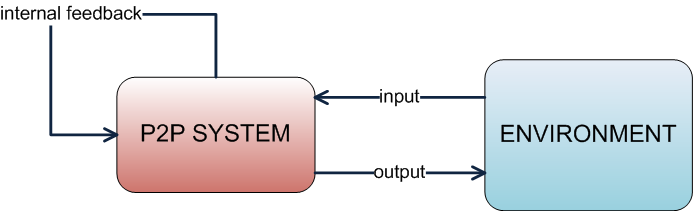
\includegraphics[width=0.5\linewidth]{imgs/5 - p2p.png}
    \label{fig:p2p}
    \caption{Struttura p2p}
\end{figure}
Gli input dell'environment targhettano pochi peer della rete.
I nodi p2p quando ricevono dei dati dalla rete possono essere progrmmati in due modi:
\begin{itemize}
    \item statico: una volta settato il nodo svolgere le sue funzioni sempre nello stesso nodo
    \item Piano adattivo: poù cambaire in corso d'opera in base a cosa gli viene detto dall'environment
\end{itemize}

\subsubsection{Variabili di stato}
Un sistema p2p è una rete di peers, quando si entra nella rete, ogni peer si connette con tutti gli altri.
I peer condividono risorse come: banda, cpu, storage, ecc.

\begin{itemize}
    \item Risorse replicabili: dati
    \item risorse consuabili: storage, cpu ecc
    \item Servizi distribuiti: servizi che rihiedono l'esecuzione su molti peer
    \item servizi locali: funzioni esposte da un peer per permettere l'accesso alle risorse locali
\end{itemize}

Ogni peer ha un tempo di vita $L$ che viene modellata secondo: il rolo del peer, disponibilità della risorsa eed eventi non predicibili.
Variabili misurate dal peer:
\begin{itemize}
    \item uso delle risorse condivise
    \item tempo di risposta dei vicini
    \item query hit ratio (QHR)
\end{itemize}

Variabili impostate dal pper:
\begin{itemize}
    \item dimensione della tabella di instradamento
    \item strategia di riempimenti delle tabelle di instradamento
    \item algoritmo per l'instradamento dei messaggi
    \item banda di unload
    \item banda download
\end{itemize}

Si usano metodi stocastici per misurare la distribuzione delle risorse e la loro popolarità.
\subsubsection{problemi di design}
La topologia della rete, il grado di centralizzazione e l'instradamento del messaggio sono cruciali per le operazioni del sistema(scalabilità, sicurezza, tolleranza agli errori, auto maantenimento).

Efficacia ed efficenza:
\begin{itemize}
    \item scalability
    \item boostrapping
    \item connectivity management
    \item search performance
    \item consitency
    \item stability
    \item load balance
    \item asymmetric bandwidth
\end{itemize}

Sicurezza:
\begin{itemize}
    \item Attacchi passivi
        \begin{itemize}
            \item eavrsdropping
            \item traffic analysis
        \end{itemize}
    \item Attacchi attvi
    \begin{itemize}
        \item spoofing
        \item man in the middle
        \item playback or replay
        \item local data alteration
        \item no forwarding
        \item free riding
        \item distributed denial of service (DDOS)
        \item network poisoning
    \end{itemize}
    \item sicurezza
    \begin{itemize}
        \item trust managment
    \end{itemize}
\end{itemize}

\subsubsection{Strategia di design per gli schemi di overlay}
nei sistemi p2p la posizione dell'informazione gioca un ruolo importante per l'overlay scheme.
\begin{itemize}
    \item server centrale
    \item peer to peer
    \item salvato in locale e non pubblico
\end{itemize}
Gli schemi di overlay:
\begin{itemize}
    \item modello ibrido(HM)
    \item modello decentralizzato non strutturato(DUM)
    \item modello decentralizzato strutturato(DSM)
\end{itemize}

\begin{figure}[h!]
    \centering
    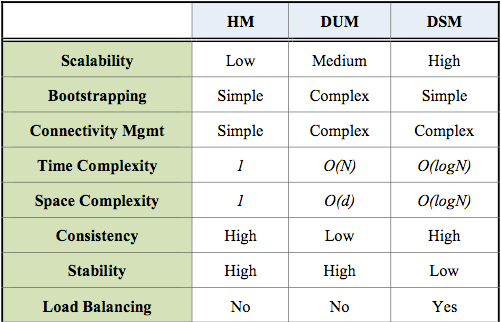
\includegraphics[width=0.8\linewidth]{imgs/6 - strategie di design p2p.png}
    \label{fig:designStrategiesP2p}
    \caption{Strategie di design reti p2p}
\end{figure}

\begin{figure}[h!]
    \centering
    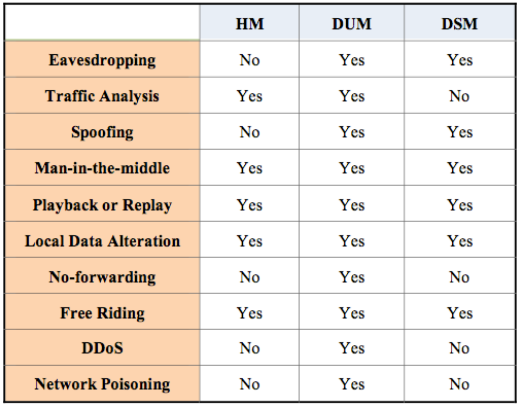
\includegraphics[width=0.8\linewidth]{imgs/7 - overlay design.png}
    \label{fig:designOverlayP2p}
    \caption{Strategie di design per gli schemi di overlay}
\end{figure}

\subsubsection{Modello ibrido(HM)}
I peer sono connessi a uno o più nodi centralizzati(server) che pubblicano le risorse.
Se un peer ha bisogno di un dato in un server, manda la richiesta, gli ritorna una risposta con il percorso da prendere e prende il dato.
Se il serve non è unico, le richieste potrebbere essere instradate a server vicini.
Esempi: eMule, BitTorret ecc
\begin{figure}[h!]
    \centering
    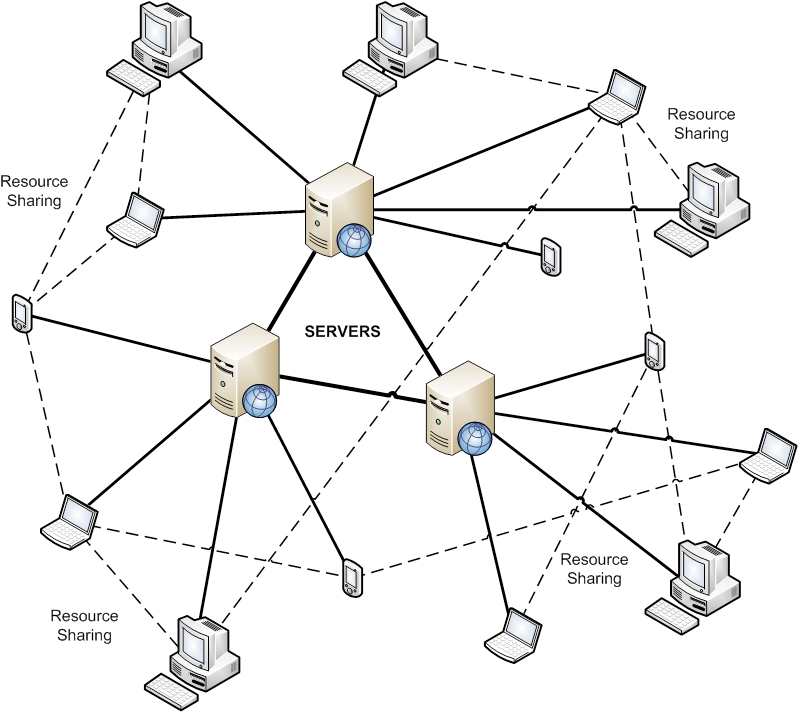
\includegraphics[width=0.5\linewidth]{imgs/8 - HM.png}
    \label{fig:p2pHM}
    \caption{Modello ibrido}
\end{figure}
\subsubsection{Modello decentralizzato non strutturato(DUM)}
Ogni peer propaga la richiesta ai peer adiacenti(simile alla strategia flooding) efficace in comunità piccole ma non scalabile.
Per migliorare la scalabilità si fa cache delle risorse recenti.
Se un'identità viene aggiunta al dato i peer possono non propagare il dato.
In network grandi è necessario un time-to-live(TTL) per evitare che un pachetto stalli per sempre.
\subsubsection{Modello decentralizzata non strutturato(DUM)}
\begin{figure}[h!]
    \centering
    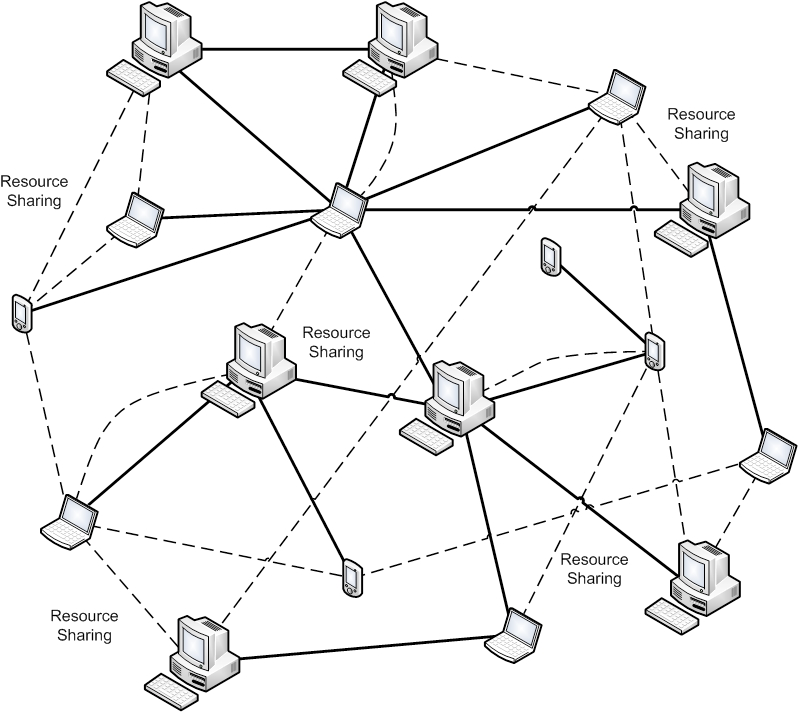
\includegraphics[width=0.5\linewidth]{imgs/9 - DUM.png}
    \label{fig:p2pDUM}
    \caption{Modello Decentralizzato non strutturato}
\end{figure}
\subsubsection{Modello decentralizzato strutturato(DSM)}

Un protocollo globale fa si che ogni noda possa raggiungere la risorsa efficacemente,
La tecnica più comune è una hash table distribuita dove ogni risorsa è identificata da una chiave univoca associata ad una chiave di decriptazione.

Ogni peer ha un ID assegnato ed è responsabile di tenere l'id salvato.

\textbf{Pubblicazione}: la descrizione di ua risorsa e la sua coppia chiave risorsa vengono messe nelle tabelle di routing adiacenti all'id del peer. 
Questo processo viene ripetuto finche ogni peer adiacente conosce l'id del peer in questione.


Il DSM è molto più decentralizzato del DUM.

\textbf{Lookup}: la query viene propagata attraverso i peer con l'ID della risorsa.

Pratica comune per stabili la lunghezza dei percorsi fra nodi è:

\begin{center}
    \begin{tabular}{| c | c |}
        \hline
        Nodi & Route Lenght \\
        \hline
        $O(1)$ & $O(N)$ \\
        \hline
        $O(\log(N))$ & $O(\frac{\log(N)}{\log(\log(N))})$ \\
        \hline
        $O(\log(N))$ & $O\log(N)$ \\
        \hline
        $O\sqrt(N)$ & $O(1)$ \\
        \hline
    \end{tabular}
\end{center}

\begin{figure}[h!]
    \centering
    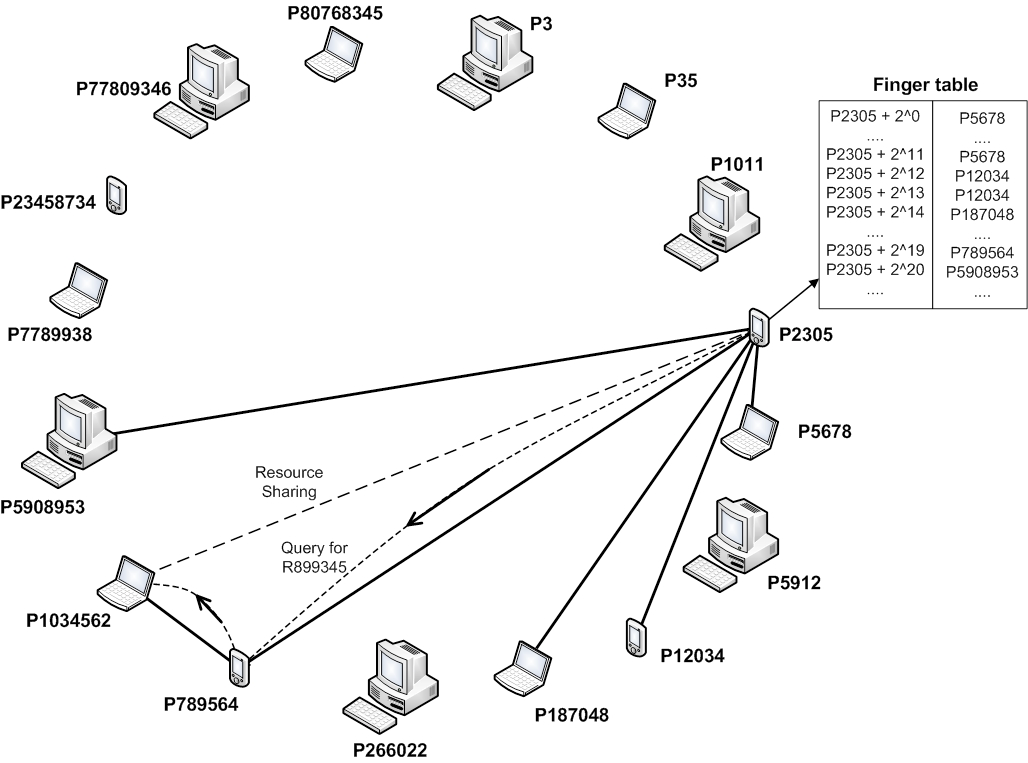
\includegraphics[width=0.5\linewidth]{imgs/10 - DSM.png}
    \label{fig:p2pDSM}
    \caption{Modello Decentralizzato strutturato}
\end{figure}

\subsubsection{Schema overaly stratificato}
In una Struttura di peers con multi layer, si utilizzano dei protocolli per permettere la comunicazione fra vari layer.

\begin{figure}[h!]
    \centering
    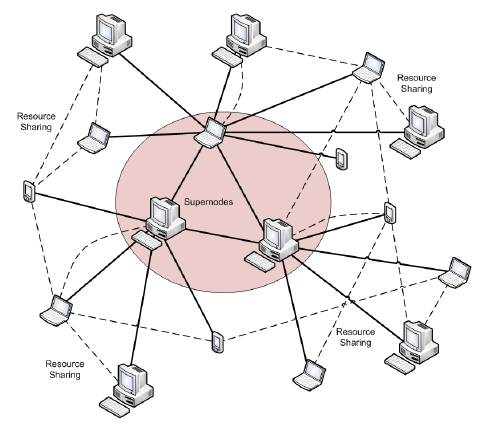
\includegraphics[width=0.5\linewidth]{imgs/11 - layer overlay scheme.png}
    \label{fig:overlay}
    \caption{Schema di overlay a strati}
\end{figure}


    %NON HO FATTO IL RIASSUNTO DELLA LETTURA, SE MI AVANZA DEL TEMPO LA FACCIO CHE SEMBRA INTERESSANTE
    \subsection{P2P - schemi di overlay popolari}
\subsubsection{Content sharing}
Gli utenti condividono i contenuti contribuend con le proprie risorse.
L'rigine della risorsa può essere da un utente o da vari.
Esempi sono:
\begin{itemize}
    \item Napster
    \item eDonkey(eMule)
    \item BitTorrent
\end{itemize}


    %SONO QUASI TUTTI ESEMPI, SE HO TEMPO LI FACCIO
    \subsection{Kademlia}
Nato nel 2002, questo protocolo si basa su DSM, utilizza delle tabelle di hash distrinuite dove ogni risorsa pubblicata viene associata ad una chiave.

\subsubsection{Distanza tra identificatori}
Kademlia usa una chiave di 160 bit per gli identificatori, nella fase di pubblicazione, la coppia chiave valore viene associata alla risorsa sulla base del id del nodo più vicino alla risorsa.
La distanza si ottiene facendo un XOR logico.
\subsubsection{Struttura dati dei nodi}
Ogni nodo ha 160 k-buckets, un bucket è una lista di massimo k tuple (indirizzi IP, UDP port, Node ID) correlate a nodi che hanno una distanza dal nodo attaule compresa tra $2^i$ e $2^{i+1}$ con i tra 0 e 159.


\begin{figure}[h!]
    \centering
    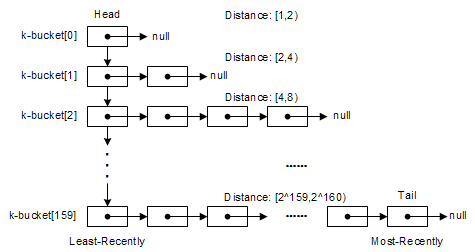
\includegraphics[width=0.5\linewidth]{imgs/12 - kbuckets.png}
    \label{fig:k-buckets}
    \caption{Esempio di struttura dei k-buckets}
\end{figure}

Quando un nodo riceve un messaggio da un'altro nodo, controlla la k-bucket che contiene la descrizione del sender, se questa descrizione è presente, il nodo muove la richiesta in coda a tutte le richieste, se la descrizione del pacchetto è assente, il noda scarta.

\subsubsection{Protocolllo RPCs}
kademlia ha 4 RPCs:

\begin{itemize}
    \item PING: il peer è online
    \item STORE: salva un dato 
    \item FIND NODE
    \item FIND VALUE
\end{itemize}

\subsubsection{Ricerca di nodi recursiva}

\begin{figure}[h!]
    \centering
    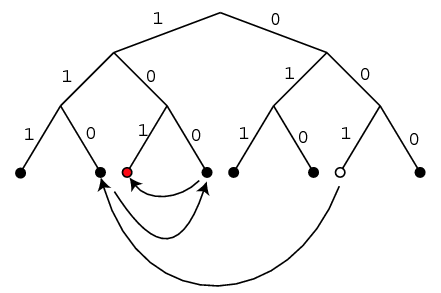
\includegraphics[width=0.5\linewidth]{imgs/13 - kademlia tree.png}
    \label{fig:kademlia-tree}
    \caption{Illustrazione del lookup dei nodi}
\end{figure}

Per publicare una risorsa (coppia chiave valore), il nodo n cerca per i k nodi vicini e invoca il metodo STORE.

Per effettuare il lookup(ricerca) della risorsa, il nodo chiama il motodo FIND VALUE di una certa chiave e propaga a tutti i nodi adiaceni, ripetere finchè non si ottiene il valore della chiave.

    \subsection{Skype}
Applicazione per fornire un servizio VOIP p2p, l'unica parte centralizzata è quella di login.
\subsubsection{Registrazione}
Durante questa parte l'utente sceglie un username $A$ e una password $P_A$.
Partendo da questi due dati, vengono generate:
\begin{itemize}
    \item Coppia di chiavi RSA $(S_A,V_A)$
    \item $S_A$ è la chiave privata
    \item $V_A$ è la chiave pubblica
    \item il peer dell'utente conserva $S_A$ e $H(P_A)$ in una cache locale sicura
    \item il peer si connette al server di login mediante una connessione basata su AES dove si generano e scambiano chiavi da 256 \begin{itemize}
    \item il peer manda al server $A, V_A $ e $ H(P_A)$
    \item il server controlla che A non sia già registrato
    \item se non registrato, procede a registrare A e $H(H(P_A))$ nel DB
    \item crea un certificato di identità $IC_A$ contenente $(A,V_A)^{S_{LS}}$ e manda il certificato al peer
    \end{itemize}
\end{itemize}

\subsubsection{Login}
\begin{itemize}
    \item Il peer si identificata con la sua IC al login server
    \item il server ritorna una lista di supernodi
    \item l'user avvia una connessione TCP
    \item il peer annuncia di ai suo peer "amici" di essere on-line
    \item i peer comunicano passando da dei supernodi(un po come dei router)
\end{itemize}

    \subsection{WebRTC e PeerJS}
\subsubsection{WebRTC}
Progetto FOSS che permette di creare browser e mobile app con comunicazione real time.
Permette di fare app come quelle per le video chiamae usando semplicemente le API di WebRTC.
\subsubsection{No plugins}
Molte app web usano WebRTC, ma necessitano di download, di plugin o app native.
\subsubsection{WebRTC app}
Un'app con WebRTC necessita di:
\begin{itemize}
    \item GET/SET streaming audio, video e di dati
    \item GET network info(IP, port) per condividerlo con gli altri per poter comunicare(anche attraverso firewall o reti NAT).
    \item Comunica segnali per gli errori
    \item scambia info riguardo le capacita del client(risoluzione, codec, ecc)
\end{itemize}

\subsubsection{STUN e TURN}
WebRTC è disegnato per lavorare con le reti p2p, ma WebRTC è costruito per funzionare nella rete tradizionale, quindi necessita di un paio di accorgimenti:
\begin{itemize}
    \item STUN per prendere l'IP del pc
    \item TURN per fare da nodi di relay se la connessione p2p fallisca
\end{itemize}

\subsubsection{Sicurezza}
La sicurezza è gestita per tutti i componenti di WebRTC, e le proprie API JavaScript possono essere usati solo con HTTP su TLS(HTTPS) o da localhost.
\subsubsection{PeerJS}
Wrappa l'implementazione browser di WebRTC per offrire una connessione p2p completa, configurabile e facile da usare.



    \section{Blockchain}
\subsection{Definizione di blockchain}
un ledger distribuito(libro mastro/contabilità) è un DB replicato su diversi nodi computazionali.
Ogni nodo ha una copa del ledger, ogni nodo che partecipa, si aggiorna autonomamente.
Non c'è un'autorità centrale, la blockchain è una forma delle tecnologie distribuite.

Una blockchain è:
\begin{itemize}
    \item un sistema che agisce come "fidato e terza parte", non centralizzato, sempre online, per mantenere un stato condiviso tramite scambi e computazioni sicure
    \item Un ledger distribuito, che salva i dati delle transazioni, raggruppate in blocchi e linkare i blocchi
    \item gestita da un grande gruppo di network servers
    \item full node: conserva una copia della blockchain, può create blocchi
    \item consensus: fra i full node, hanno gli stessi blocchi
    \item wallet: software per fare transazioni
    \item public = permissionless: tutti possono
        \begin{itemize}
            \item essere un utente
            \item fare transazioni
            \item partecipare al consenso
        \end{itemize}
    \item private = permissioned: le operazioni della blockchain possono essere fatte da membri autorizzati, full node identificabili, regole per l'accesso dei dati
\end{itemize}

\subsection{P2P Network}

I full node collaborativamente mantengono una rete p2p per lo scambio di blocchi e scambi di transazioni.

Le regole del consenso non coprono la parte di networking, i full node
possono usare protocolli orienteti alla velocità fra di loro le varie transazioni.

Al primo avvio di una applicazione, questa non consoce l'IP di nessun full node, effettua una query
ad un server DNS, questa query prende il nome di DNS seeds, che risponde all'applicazione con il lookup e
un indirizzo IP di un full node che accetta nuove connessioni.

Per validare una transazione, un full node deve aver scaricato tutti blocchi della blockchain per poter
aggiungere un nuovo blocco di transazioni.

Quando viene scoperto un nuovo blocco, questo viene inviato a tutti i peer della rete 
mediante la "Block Broadcasting".

\subsection{Motivi per usare una blockchain}
\begin{figure}[h!]
    \centering
    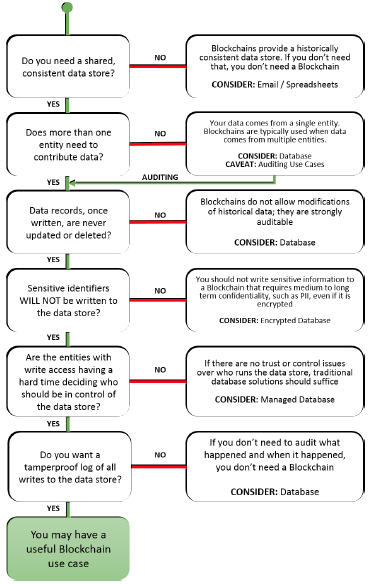
\includegraphics[width=0.5\linewidth]{imgs/14 - motivi uso blockchain.png}
    \label{fig:why_use_blockchain}
    \caption{Usi di una blockchain}
\end{figure}

\subsection{Coin vs Token}
Parlando di criptovalute associate a blockchain, si distinguono:
\begin{itemize}
    \item Coin: unità di valuta della blockchain, usata per le transazioni
    \item Token: unità secondaria che risiede nella blockchain con vari scopi:
        \begin{itemize}
            \item utility tokens: rappresentano il diritto di prendere prodotti/servizi dall'emittente del token
            \item security tokens: asset digitali il cui valore deriva da quanto questo asset viene scambiato
        \end{itemize}
\end{itemize}

Il security token potrebbe essere visto come "un'azione in borsa", può generare interesse, ecc


\subsection{Transazioni}
Le transazioni rappresentano pagamenti per beni o servizi utilizzando i "coins", 
le parti vengono identificate da chiavi pubbliche e 
ogni pagamento viee firmato digitalmente.

\subsection{Bitcoin}
\begin{itemize}
    \item Blocco di genesi: 3 Gennaio 2009
    \item developer: "Satoshi Nakamoto", Gavin Andresen, Wladimir van der Laan
    \item 1 BTC = $10^8$ satoshi
\end{itemize}

Le valte basate sulla blockchain, vengono generate tramite un processo decentralizzato e competitivo
detto mining.
I miners di bitcoin sono i full node che processano le transazioni e rendono sicuro il network.

C'è un numero limitato di bitcoin in circolo e i bitcoin vengono generati con un andamento 
prevedibile(mantenendo il prezzo stabile).

Visto che il marketcap di bitcoin è ancora piccole, quantità di denaro elevate possono far oscillare il prezzo.



\begin{figure}[h!]
    \centering
    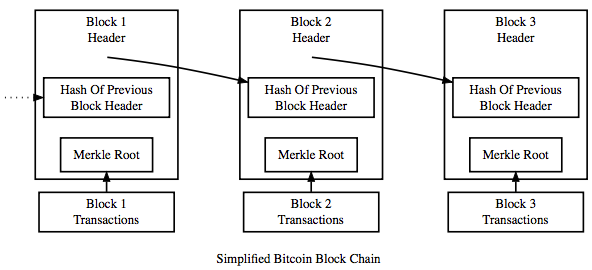
\includegraphics[width=0.5\linewidth]{imgs/15 - bitcoin block.png}
    \label{fig:bitcoin_block}
    \caption{Struttura Blocco bitcoin}
\end{figure}

Ogni blocco di transazioni, vengono "hashate" nel \textbf{Merkle tree}, finchè la hash unica(\textbf{Merkle Root}) 
viene prodotta e salvata nell'header del blocco, insiseme all'hash del header del blocco precedente.

\subsubsection{Merkle Tree}

\begin{figure}[h!]
    \centering
    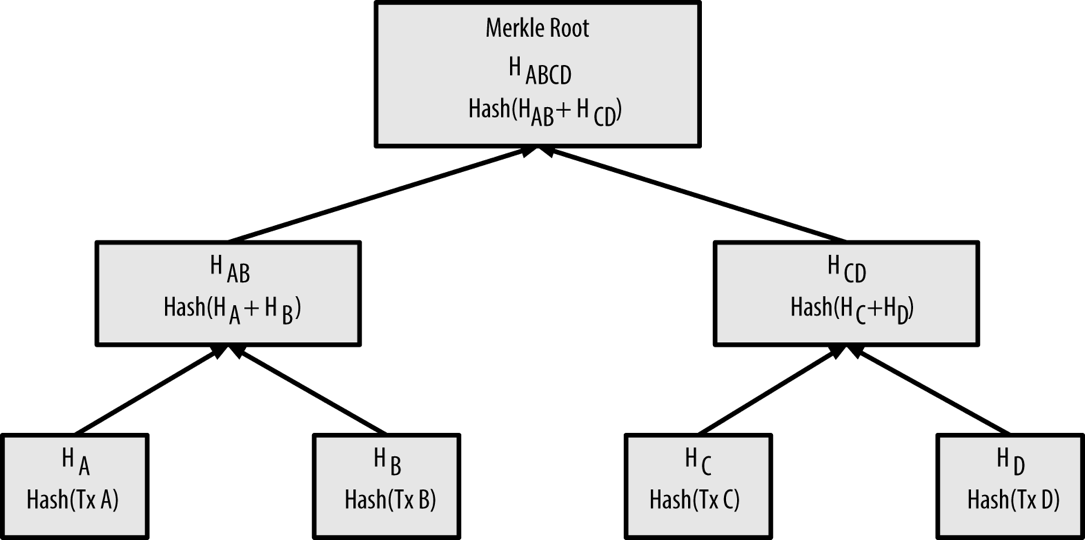
\includegraphics[width=0.5\linewidth]{imgs/16 - merkle tree.png}
    \label{fig:merkle_tree}
    \caption{Merkle Tree}
\end{figure}


Il merkle tree viene creato facendo l'hash di blocchi accoppiati (le foglie dell'albero),
Viene ripetuto il procedimento di pairing e hashing finchè non rimane una sola hash.

\subsubsection{Transazioni Bitcoin}
\begin{itemize}
    \item Tutte le transazioni sono collegate
    \item \textbf{input}: riferimeto al blocco precedente
    \item \textbf{output}: quantità di valuta da trasferire
    \item ogni transazioni ha più di un input e più di un output
    \item Se l'output è maggiore del'input, la transazione è annullata
    \item se il sender invia 50 ma il reciver vuole 25, ci saranno due transazioni da 25 di cui una sarà il "resto"
    \item il ricevitore invia la chiave pubblica al pagatore
    \item il pagatore crea la transazione, specificando l'output e la firma(hash della chiave pubblica del reciver)
    \item il payer firma la transazione con la propria chiave privata
    \item la transazione viene inviata dal sender alla rete di full node
    \item il full node verifica la transazione e se valida la aggiunge alla blockchain
\end{itemize}

\subsection{Smart contract}
\begin{itemize}
    \item Programma salvato nella blockchain
    \item espressione di logica contrattuale
    \item può implementare ogni algoritmo
    \item comportamento deterministico
    \item può interagire con altri contratti
    \item rende pubblica un'interfaccia
    \item può ritornare dati o salvare dati
    \item il messasggio può rappresentare eventi di interesse del contratto
    \item le interazioni con gli smartcontract sono salvate in blockchain
    \item DApp (applicazione decentralizzata): frontend + decentralized logic
    \item ICO (initial coin offering): crowfounding per un progetto, in cambio di coins specifici
    \item DAO (decentralized anonymous organization): organizzazione anonima amministrata da uno smart contract
\end{itemize}

\subsubsection{Concorrenza e smart contract}

\textbf{contracts-as-comcurrent-objects analogy}: account che usano gli smart contract in una blockchain sono come i threads di un pc.

\subsection{Ethereum}
\begin{itemize}
    \item Si può usare un'implemetazione di go
    \item 60 milioni di ether creti grazie ai contributori del presale
    \item 12 miglioni dati alla fondazione, ai finanizatori e ai dev
    \item 5 theters crati ogni blocco(13 sec per minare un blocco)
\end{itemize}

\subsubsection{Ethereum accounts}
Due tipologie di account in ethereum:
\begin{itemize}
    \item normale: controllato da coppie di chiave pubblica
    \item contratto: controllato dal codice interno
\end{itemize}

Chiavi private da 256 bit e pubbliche da 512 bit, vengono generate per ogni account.

\subsubsection{Smart contract ethereum}
Ogni smart contract ha un indirizzo unico, assegnato da una transazione speciale, dopo la quale, il programma fa parte della blockchain.
Per compie una interazione, bisogna mandare un messaggio all'indirizzo del contratto.
I contratti possono avere stato e memoria interna.

I contratti ethereum vengono scritti in \textbf{Solidity}(simile a javascript), compilato ed esequito nella ethereum virtual machine(EVM).

\begin{itemize}
    \item \textbf{kovan, ropsten}: testnet
    \item \textbf{truffle}: framefork(test i contratti in locale)
    \item \textbf{ganache}: crea una blockchain locale per test
\end{itemize}

Ogni operazione effettuta da un contratto, ha un costo.
\begin{itemize}
    \item TX = tassa totale operazione
    \item GU = gas usato per l'operazione
    \item GP = prezzo del gas
\end{itemize}

\begin{math}
    TX = GU * GP
\end{math}

E operazioni diverse hanno un consumo diverso di gas.

Il gas limit è il limite è il limite per il quale si è decisi di pagare.
Impostare un gas limit troppo alto risulta meno interessante per i miners, che cercano di massimizzare i guadagni per ogni songolo blocco.

I miner guardano il prodotto tra gas price e gas limit per vedere quale contratto è più remunerativo.

\subsubsection{Verifica di Merkle in ethereum}
In ETH, lo stato è un'enorme struttura dati chiamata \textbf{modified merkle patricia trie}, gli header di ogni blocco 
contengono tre merkle tree(transazioni, receipts(ricevute? e lo stato)).

\begin{figure}[h!]
    \centering
    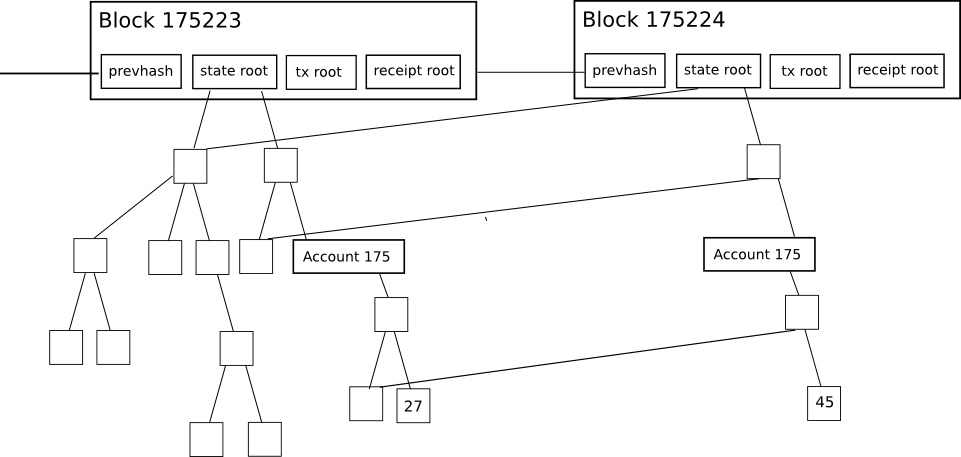
\includegraphics[width=0.5\linewidth]{imgs/17 - merkle tree.png}
    \label{fig:merkle_proof}
    \caption{Applciazione del Merkle tree}
\end{figure}

Bitcoin usa un albero binario, in ETH, usando l'albero di merkle si possono ottenere struttre molto complesse come
Transazioni richieste, transazioni in uscita e gli stati dell'account.

Si utilizaz il Merkle patricia tree perchè permette:
\begin{itemize}
    \item Calcolo facile del nuovo albero dopo la modifica
    \item La profondità dell'albero e vincolata
    \item la radice dipende solo dai dati(non l'ordine degli aggiornamenti)
\end{itemize}



\subsection{Modelli di consenso}
Principio importante della blockchain è chi è l'utente a creare un nuovo blocco.

In blockchain "permissionless", ci sono vari nodi che creano blocchi che competono per il blocco.
Fanno il nuovo blocco per vincere criptovalute.

Motivati dal guadagno.


Le seguenti proprietà sono in gioco:
\begin{itemize}
    \item Si parte dal blocco di genesi
    \item gli utenti sono daccordo con il modello di consenso sui blocchi creati
    \item ogni blocco è linkato al precedente mediante un hash
    \item ogni utente può verificare i blocchi.
\end{itemize}

I modelli di consenso comuni sono:
\begin{itemize}
    \item Proof of work
    \item Proof of Stake
    \item Round Robin
    \item Proof of Authority/Proof of Identity
    \item Proof of Elapsed Time
\end{itemize}

\subsubsection{Proof of Work(PoW)}
I full node competono a creare il nuovo blocco.
Spesso si utilizzano gli ASIC, PC specilizzati in fare coalcoli per la creazione dei blocchi.
Clacolano l'hash di alcuni dati finchè il risultato è simile alla traccia, il primo nodo che finisce l'operazione, propone il nuovo blocco nella blockchain.

Per ogni blocco aggiunto il full node prende una ricompensa in criptovalute.

La difficolta del problema di hash viene ricalcolato continuamente per mantenere lo stesso tempo stabile fra ogni blocco creato.


In Bitcoin, SHA-256 crea una hash del merkle tree + blocco precedente + header + random finchè il risultato non rispetta la soglia.

I nuovi blocchi vengono aggiunti solo se risolvere la loro hash era difficile quanto stabilito dal metodi di consenso.
Ogni N blocchi (N = 2016 in bitcoin), la sogni di difficoltà si ribilancia calcolando il tempo tra il primo e l'ultimo blocco.

In ETH l'algoritmo si chiama \textbf{Ethash}, la funzione per minare combina e fà l'hash (Keccak-256) di: random, hash dell'header del blocco e dati random del set.

L'algoritmo itera finchè la soglia non è raggiunta.

Il "Miner" che raggiunge l'hash di difficoltà accettata dalla soglia, prende la commissione, aggiunge il blocco alla blockchain e diffonde la notizia.

Non conviene aggiungere tante trasazioni in un blocco perchè rallenta la creazione del blocco.


Se qualcuno possiede il $51\%$ di hash rate della blockchain, potrebbe modificare le transazioni e evitare che nuove transazioni vengano fatte.

Se due nodi creano un blocco nello stesso momento, la chain si biforca e se nella blockchain 2 viene aggiunto un nuovo blocco, questa seconda chain diventa più affidabile della prima poichè più difficile da ricreare(ha un blocco in più).

\begin{figure}[!ht]
    \centering
    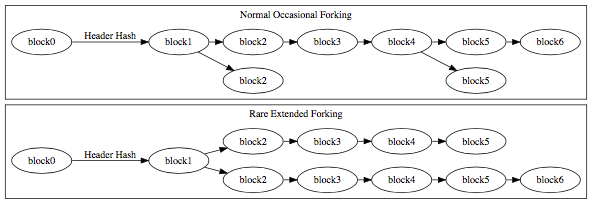
\includegraphics[width=0.5\linewidth]{imgs/18 - fork.png}
    \label{fig:fork}
    \caption{Biforcazione della blockchain}
\end{figure}

PoW è molto dispendiosa in quantità di energia.


\subsubsection{Proof of Stake(PoS)}

La blockchain mantiene proprietà di una popolazione di coins "staked" dai partecipanti.
Per aggiungere un blocco, la probabilità di creare un nuovo blocco aumenta se si hanno più coins in stacking.

Vantaggi:
\begin{itemize}
    \item minor rischio di centralizzazione
    \item efficienza energetica
\end{itemize}

Svantaggi:
\begin{itemize}
    \item eleggere il creatore del blocco implica randomicità
    \item brecce di sicurezza.
\end{itemize}

Gli attaccanti possono fare l'hash dell'intera blockchain per sferrare l'attacco "grinding attack".

\subsubsection{Eventual-consensus PoS protocols}
Questo protocollo applcia una forma di "longest-chain
rule" alla blockchain, l'immutabilità della blockchain aumenta con la quantità di blocchi.

\subsubsection{Blockwise-BA PoS protocols}
Questo protocollo ottiene l'immutabilità di ogni singolo blocco mediante il protocollo \textit{Byzantine Agreement}.

Esempio: ALGORAND


\subsubsection{Problema di non avere stacking}
Visto che la validazione dipende dallo stacking, non avere stacking porta problemi come la Biforcazione.

Portando a fenomeni come il double spending, competizione per blocchi su catene diverse ecc.

\subsubsection{Attacco a lungo termine}
Legato al concetto di creare "brench" senza sforzo, si riferisce alla capacità di alcuni set di stackholders di eseguire la blockchain
dal blocco di genesi e produrre una alternativa alla blockchain.

Due attacchi:
\begin{itemize}
    \item posterior corruption
    \item stake-bleeding
\end{itemize}

Per evitare i long range attack:
\begin{itemize}
    \item checkpoints: gli ultimi K blocchi possono essere riorganizzati
    \item valutazione della chiave crittografica
    \item restrixioni della densita della chain
\end{itemize}

\subsubsection{Blockchain $\approx$ Merkle hash function}
La struttura della blockchain è molto simile allo schema di merkle per la funzione di hash, dove la compressione è iterata su un messaggio che viene processato in blocchi.

La funzione di hash di Merkle deve soddisfare tre proprietà di sicurezza:
\begin{itemize}
    \item preimage resistance
    \item second preimage resistance
    \item collision resistance
\end{itemize}

\subsubsection{Eclipse attack}
L'attacco opera al livello della rete p2p, un nodo sotto attacco ottiene una vista distorta della blockchain perchè l'attaccante controlla le comunicazioni.

\subsubsection{Riassunto delle possibili falle di sicurezza}
PoW:
\begin{itemize}
    \item 51$\%$ attack
\end{itemize}

PoS:
\begin{itemize}
    \item Nothing at Stacke
    \item Long-Range attack
\end{itemize}

Problemi generali:
\begin{itemize}
    \item second preimage attack
    \item Eclipse attack
\end{itemize}

\subsubsection{Modello di consenso Round Robin}
Usato da network \textbf{Permissioned}, non ha puzzle crittografici e ha una potenza richiesta ridotta.
I nodi a turno creano i blocchi ed è presente un timeout per prevenire che nodi in "stallo" alterino la crescita della blockchain.

\subsubsection{Modello di consenso Proof of Authority/Proof of Identity}
I nodi che creano blocchi devono avere un'identità verificata e hanno una reputazione da preservare, minore è la reputazione, minore sono le possibilità di creare blocchi.
Utilizzabile solo nelle reti \textbf{permissioned}

\subsubsection{Proof of Elapsed Time(PoET)}
Ogni nodo richiede un timer di attesa all'\textbf{hardware time source}, l'hardware genera il tempo di attesa
e una volta ricevuto il timer, vanno in idle.
Una volta ripartito dall'idle, il nodo, crea un blocco, tutti gli altri blocchi interrompono l'idle e il processo riparte.

Utilizzabile in network \textbf{Permissioned e trusted}.
\end{document}